%!TEX root = ../report.tex
\section{Changing grid resolution}

In order to check whether the accuracy of the solutions is adequate, we change the resolution of the model. We have computed the steady states in $\eta = 1$ and $Re = 16$ for grid resolutions $32\times 32$, $64\times 64$, $96\times 96$, $128\times 128$ and $160\times 160$. In Figure~\ref{fig:grids} the resulting streamfunctions are shown for three grid sizes. A quick look tells us that the shapes of the solutions are qualitatively the same. 

\begin{figure}[h]
    \centering
    \begin{subfigure}[b]{0.6\textwidth}
        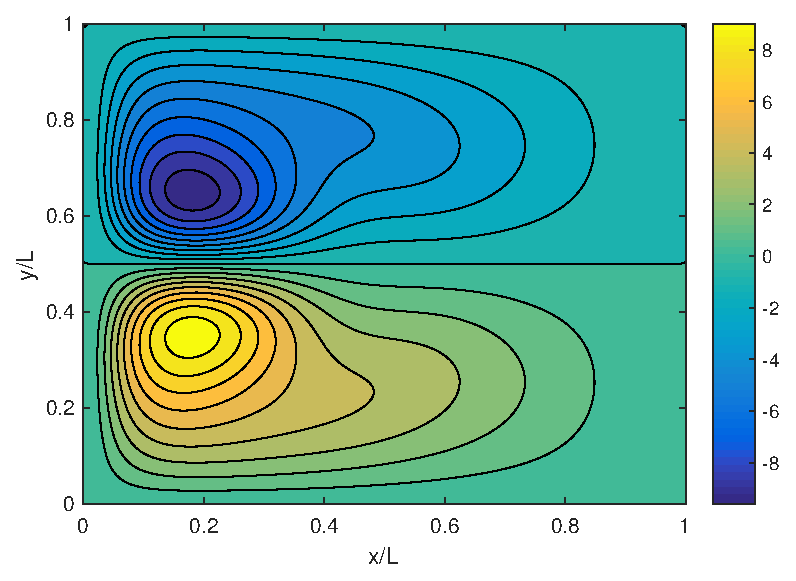
\includegraphics[width=\textwidth]{images/grid128.eps}
        \caption{$128\times 128$}
        \label{fig:nm128}
    \end{subfigure}
    \centerline{
    \begin{subfigure}[b]{0.5\textwidth}
        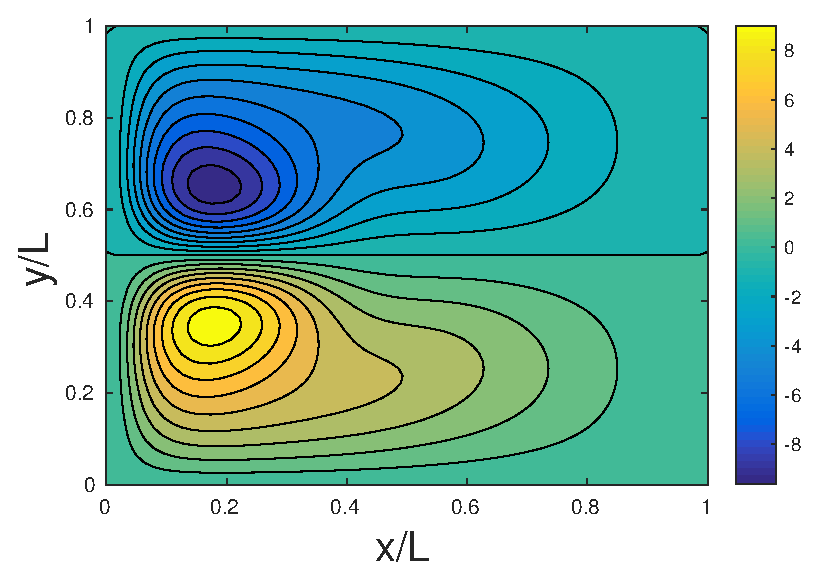
\includegraphics[width=\textwidth]{images/grid64.eps}
        \caption{$64\times 64$}
        \label{fig:nm64}
    \end{subfigure}
    ~
    \begin{subfigure}[b]{0.5\textwidth}
        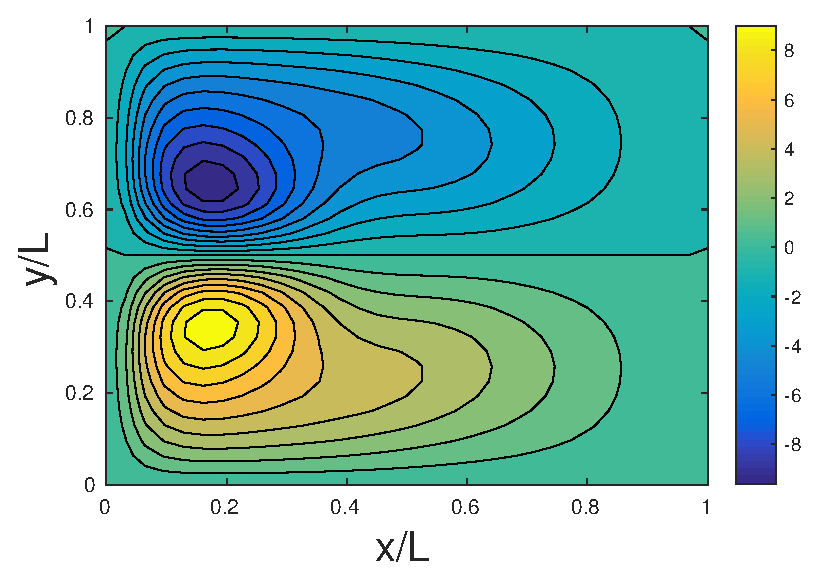
\includegraphics[width=\textwidth]{images/grid32.eps}
        \caption{$32\times 32$}
        \label{fig:nm32}
    \end{subfigure}
    }
    \caption{$\psi$ at $Re = 16$ for different grid sizes.}\label{fig:grids}
    
\end{figure}

\begin{figure}
	\centerline{\includegraphics{images/errors.pdf}}
	\caption{Approximate errors (differences to the extrapolant) for multiple values of interest. We see clearly second order convergence in the global error; locally we see that the higher order terms still play a role when $n < 128.$}
	\label{fig:errors}
\end{figure}

For a more accurate approach, we compute an approximate error using a higher-order guess for local values $\psi(\tfrac{1}{8}, \tfrac{1}{8}),$ $\psi(\tfrac{3}{8}, \tfrac{3}{8})$ and the global norm $\|\psi\|_\infty.$ The basic trick is as follows: given two $k$th order approximations $f(h)$ and $f(ah)$ to a value $f^*,$ we can compute a $(k+1)$th order approximation to $f^*$ as follows:
\begin{align}
    f(h) &= f^* + C h^k + O(h^{k+1}), \label{eq:a} \\
    f(ah) &= f^* + C a^k h^k + O(h^{k+1}) \label{eq:b}
\end{align}
Subtracting~\eqref{eq:b} from $a^k \times$~\eqref{eq:a} gives a $(k+1)$th order approximation to $f^*$ of the form
\begin{equation}
    f^* = \frac{a^k f(h) - f(ah)}{a^k - 1} + O(h^{k+1}).
\end{equation}
Since we have a second-order discretization we take $k = 2,$ and then apply the Richardson extrapolation to the grids of $n = 128$ and $n = 160.$ The resulting values are listed in Table~\ref{table:extrap}. Next we use these extrapolations to plot the approximate error in Figure~\ref{fig:errors}, where the straight line ($\sim/N^2$) is a reference to determine whether the accuracy is indeed second order. We see for grid sizes around $128 \times 128$ that the solution is approximately second order accurate as desired.

\begin{table}[t]\centering
\ra{1.3}
\begin{tabular}{@{}rrrr@{}}\toprule
  & $\psi(\tfrac{1}{8}, \tfrac{1}{8})$ & $\psi(\tfrac{3}{8}, \tfrac{3}{8})$ & $\|\psi\|_\infty$\\ \midrule 
$n = 32$                 & 0.327567 & 0.500404 & 1.02851\\
$n = 64$                 & 0.381462 & 0.489258 & 1.07422\\
$n = 128$                & 0.410911 & 0.476320 & 1.08405\\
$n = 160$                & 0.416887 & 0.472971 & 1.08572\\ \midrule
Extrapolation      & 0.427511 & 0.467017 & 1.08869\\ \midrule
Relative error $n = 32$  & 31\%     & 6.7\%    & 5.85\% \\
Relative error $n = 64$  & 12\%     & 4.5\%    & 1.35\% \\
Relative error $n = 128$ & 4.0\%    & 2.0\%    & 0.43\% \\
Relative error $n = 160$ & 2.5\%    & 1.3\%    & 0.27\% \\
\bottomrule
\end{tabular}
\caption{Richardson extrapolation of interesting values. Note that the relative errors are only approximate and taken with respect to the extrapolated number.}\label{table:extrap}
\end{table}

Lastly, we have listed the approximate relative errors of the quantities with respect to the extrapolations in Table~\ref{table:extrap} as well. Starting at $n = 128$ we see a relative error less than $5\%$ not only locally at the two points of interest, but as well globally in the infinity norm. Although it completely depends on the use case, we think a $128 \times 128$ grid and larger is by the above arguments Good Enough\textsuperscript{TM}.